\documentclass[draft]{uw-ece-wkrpt}
\usepackage[no-math]{fontspec}
\usepackage[hidelinks]{hyperref}
\usepackage[backend=biber,style=ieee]{biblatex}
\usepackage[xindy,toc,nopostdot]{glossaries}
\usepackage{graphicx}
\usepackage{amsmath}
\usepackage[binary-units]{siunitx}
\usepackage[final]{listings}
\usepackage[dvipsnames]{xcolor}
\usepackage{tabularx}
\usepackage{booktabs}
\usepackage[tableposition=top]{caption}
\usepackage{float}

\usepackage[firstpage]{draftwatermark}
\SetWatermarkText{DRAFT}

\sisetup{detect-all}
\lstset{
    frame=single,
    basicstyle=\footnotesize,%\fontspec{Menlo}\footnotesize,
    tabsize=4,
    commentstyle=\color{CadetBlue},    % comment style
    keywordstyle=\bfseries\color{OliveGreen},       % keyword style
    stringstyle=\color{WildStrawberry},     % string literal style
    %numberstyle=\tiny\color{mygray}, % the style that is used for the line-numbers
    belowcaptionskip=10pt,
}

\setmainfont{Times New Roman}
\makeglossaries

%%% Acronyms %%%

\newacronym[%
    description={Convolutional Neural Net, a deep, feed-forward neural network implemented generally for image recognition; uses convolution operations.}%
]{cnn}{CNN}{Convolutional Neural Net}

\newacronym[%
    description={Directed Acyclic Graph, a graph with directed edges that also contains no cycles.}%
]{dag}{DAG}{Directed Acyclic Graph}

\newacronym[%
    description={Field Programmable Gate Array, an integrated circuit containing programmable logic cells.}%
]{fpga}{FPGA}{Field Programmable Gate Array}

\newacronym[%
    description={Intellectual Property, specifically referring to vendor-designed circuit blocks.}%
]{ip}{IP}{Intellectual Property}

\newacronym[%
    description={Logic Element, a unit of programmable logic cell implementing Boolean functions.}%
]{le}{LE}{Logic Element}

\newacronym[%
    description={Multiply-Accumulate, an operation performed by a convolution, computable as an inner product of two matrices.}%
]{mac}{MAC}{Multiply-Accumulate}

\newacronym[%
    description={Peripheral Component Interconnect Express, a high-speed data connection between system components such as CPU and memory and external components such as FPGAs and graphics cards.}%
]{pcie}{PCIe}{Peripheral Component Interconnect Express}

\newacronym[%
    description={Random Access Memory. Data storage that can be arbitrarily addressed efficiently.}%
]{ram}{RAM}{Random Access Memory}

\newacronym[%
    description={Block RAM. A type of memory block in FPGA fabrics that can be linked together to create memoriy banks of various dimensions.},%
    see={ram}%
]{bram}{BRAM}{Block RAM}

\newacronym[%
    description={Dynamic RAM. RAM that cannot retain data indefinitely and requires periodic ``refreshing,'' where the data contents are read and re-written (compare with SRAM).},%
    see={ram,sram}%
]{dram}{DRAM}{Dynamic RAM}

\newacronym[%
    description={Static RAM. RAM that retains its data so long as it is powered (compare with DRAM).},%
    see={ram,dram}%
]{sram}{SRAM}{Static RAM}

\newacronym[%
    description={Read Only Memory. Data storage that is programmed once on creation of the ROM.}%
]{rom}{ROM}{Read Only Memory}

\newacronym[%
    description={Rectified Linear Unit, a common activation function defined as $f(x) = \max(0, x)$.}%
]{relu}{ReLU}{Rectified Linear Unit}

\newacronym[%
    description={Register Transfer Level, a language which describes hardware elements at the register level.}%
]{rtl}{RTL}{Register Transfer Level}

\newacronym[%
    description={Robot Operating System, a framework for sensors, actuators, and processors to communicate.}%
]{ros}{ROS}{Robot Operating System}

\newacronym[%
    description={Very-Large-Scale Integration, the technology of integrating a very large number of transistors (today billions) on a single piece of semiconductor, typically silicon.}%
]{vlsi}{VLSI}{Very-Large-Scale Integration}

%%% Glossary entries %%%

\newglossaryentry{bias}
{
    name=bias,
    description={A neural network parameter that is added to the result of a kernel convolution.}
}

\newglossaryentry{conv_window}
{
    name=convolution window,
    description={The region in an input matrix being multiplied by the kernel.}
}

\newglossaryentry{filter}
{
    name=filter,
    description={Synonym for kernel.},
    see={kernel}
}

\newglossaryentry{kernel}
{
    name=kernel,
    description={a matrix of size n x n that is moved over the input image, taking the inner product with the input feature map to generate a point in the output feature map .}
}

\newglossaryentry{neural_net}
{
    name=neural network,
    description={Neural Network, a data processing paradigm that was inspired by the way the human brain processes information.}
}

\newglossaryentry{tensor}
{
    name=tensor,
    description={A generalized vector or matrix that could be of higher dimensions; represented as an n-dimensional array.}
}

\newglossaryentry{weight}
{
    name=weight,
    description={The value of an individual entry of a kernel.}
}

\addbibresource{nn2rtl_final_report.bib}

\title{RTL Generator and Optimizer for Implementation of Neural Networks on FPGAs}
\author{Minghao Ji (20549008)\\
        Pragash Sivasundaram (20568317)\\
        Timothy Chee Tim Mui (20573097)\\
        Tong Su (20563121)\\
        Yifei Li (20570146)}
\group{Group 2019.045}
\school{University of Waterloo}
\faculty{Faculty of Engineering\\Department of Electrical and Computer Engineering}
\consultant{Prof. Derek Rayside}
\date{Jan 10, 2019}

\begin{document}

\maketitle

%%%%%%%%%%%%%%%%%%%%%%%%%%%%%%%%%%%%%%%%%%%%%%%%%%%%%%%%%%%%%%%%%%%%%
%% FRONT MATTER
%%%%%%%%%%%%%%%%%%%%%%%%%%%%%%%%%%%%%%%%%%%%%%%%%%%%%%%%%%%%%%%%%%%%%
%% \frontmatter will make the \section commands ignore their numbering,
%% it will also use roman page numbers.
\frontmatter

\begin{onehalfspacing}

\section{Abstract}
As \glspl{neural_net} become increasingly portable, accelerators such as \glspl{fpga} are more prevalent over General Purpose GPUs given strict energy and performance constraints. A recent study by Intel shows that their Arria 10 \gls{fpga} offers a 16\% better performance/watt over GPU for matrix arithmetic operations that are integral to \glspl{neural_net}. However, implementing a \gls{neural_net} on an \gls{fpga} requires multiple iterations of optimization, pruning and hardware generation\textemdash{}often done ad hoc by developers. This project enables developers to specify the parameters of a trained \gls{neural_net} through Google's open-source TensorFlow syntax. The syntax is parsed as a graph structure, with each node representing a neuron in the \gls{neural_net}. The graph is quantized and optimized automatically, for the purpose of saving \gls{fpga} area and performance. The optimized graph is used to generate \gls{rtl} Verilog that can be compiled into hardware. For developers with less hardware design experience, this tool will lower the technical knowledge required to leverage \glspl{fpga} for \glspl{neural_net}. For expert hardware designers, this tool can significantly reduce the developer hours required to implement and iterate a \gls{neural_net} design on an \gls{fpga}.

\clearpage
\section{Acknowledgements}
We would like to acknowledge the many people who helped our team design, build, and test our project. A multi-disciplinary project such as this one would not be possible without the help of the following people:

\begin{flushleft}
\begin{tabular}{l@{\hskip 3cm}l}
    Consultant       & Prof.\@ Derek Rayside \\
    \\
    Faculty Advisors & Prof.\@ Nachiket Kapre \\
                     & Prof.\@ Sagar Naik \\
    \\
    WATonomous Team  & David Murdoch \\
                     & Ankil Patel \\
                     & Simon Fan \\
                     & Kenneth Jung \\
                     & Anish Chopra \\
                     & Jason Milasincic \\
    \\
    Intel Corporation & Blair Fort \\
\end{tabular}
\end{flushleft}

We have been very fortunate to have subject matter experts, such as the ones above, who have shared their knowledge with us and have been helping with any requests from our team. We would also like to thank our family, friends, and all who have supported our project.

\end{onehalfspacing}

\tableofcontents
\listoffigures
\listoftables
\addcontentsline{toc}{section}{Listings}
\lstlistoflistings

%%%%%%%%%%%%%%%%%%%%%%%%%%%%%%%%%%%%%%%%%%%%%%%%%%%%%%%%%%%%%%%%%%%%%
%% REPORT BODY
%%%%%%%%%%%%%%%%%%%%%%%%%%%%%%%%%%%%%%%%%%%%%%%%%%%%%%%%%%%%%%%%%%%%%
%% \mainmatter will make the \section commands numbered again,
%% it will also use arabic page numbers.
\mainmatter
\glsresetall

\section{Project Description}

\subsection{Motivation}

Neural networks are becoming an increasingly common solution in various domains, capable of anything from facial recognition algorithm on phones \cite{Stoimenov2016Face-recognitio} to navigation and image recognition on autonomous vehicles \cite{Ucar2017Object-recognit}. Large strides taken by Alex Krizhvevsky et al. at the University of Toronto in this field have paved the way for more complex and performant \glspl{neural_net} \cite{Krizhevsky2017ImageNet-Classi}. Hardware limitations have traditionally acted as a bottleneck; but the evolution of CPUs, GPUs and \glspl{fpga} have curbed this issue.

\glspl{fpga} remain the most energy efficient solution of the three, making it the optimal solution for mobile deployment of \glspl{neural_net}. However, a significant issue facing the developers today is the steep learning curve and long iteration times required when designing for \glspl{fpga}. Often developers are interested in accelerating a \gls{neural_net} solving a domain specific problem and are agnostic to the implementation of the \gls{neural_net} on the \gls{fpga}, if it meets certain speed requirements. Currently, developers are forced to implement their own ad-hoc script to optimize and compile their model onto an \gls{fpga}. There has been recent development of tools for generating \gls{rtl} implementation of \glspl{neural_net} for \gls{fpga} \cite{Ma2017An-automatic-RT}.

TensorFlow also provides tools for optimizing \gls{neural_net} models. However, the interaction between the effects model optimization and hardware optimization is not captured in either of these tools. When accelerating a \gls{neural_net} through \gls{fpga}, hardware generation phase is often in the critical path of the project and allowing for it to be started earlier in the design process will be a significant advantage.

\subsection{Project Objective}

The objective of this project is to design a generalized tool that accepts a trained \gls{neural_net} and a list of configurations from a user, and output \gls{rtl} code that is deployable for an \gls{fpga}. This will allow developers and system architects a simple and fast tool to enable hardware acceleration in their systems with minimal additional investments. An additional feature will be network optimization performed by the tool before \gls{rtl} output. Model compression to directly improve the output hardware will be executed before an optimized hardware architecture is generated. This tool will hopefully enable more systems to take advantage of the performance gains that can be achieved by utilizing hardware acceleration.

This tool will be built in collaboration with WATonomous (WATO) student design team at the University of Waterloo to accelerate the image recognition and classification algorithm for an autonomous vehicle. Because of this, the trained model and the integration of the \gls{fpga} into the vehicle will be completed by WATO.

\subsection{Block Diagram}

The primary components of the system, as seen in Figure \ref{fig:system_block_diagram}, are Front End, Middle End, and Back End. The Front End consists of the User Interface module and TensorFlow Model Ingestion. The parsed \gls{neural_net} is then passed to the Middle End. The Middle End consists of two main blocks: Model Compression and Hardware Gen. The next block Hardware Gen offers three functionalities: model analysis, schedule generation and macro generation.  The detailed design of each module is expanded upon later in the report.

The system maintains two representations of the target \gls{neural_net}: one in abstract form describing nodes and connectivity (in blue), and a second hardware-mapped form produced by hardware architecture generation (in red).

Figure \ref{fig:system_block_diagram} also shows how the output of the \gls{rtl} generation will be used by an \gls{fpga} CAD tool. This tool would be provided by the \gls{fpga} vendor, such as Intel/Altera or Xilinx. The \gls{rtl} will be compiled by the \gls{fpga} tool and make up the Generated Core Engine on the \gls{fpga}.

\begin{figure}
    \centering
    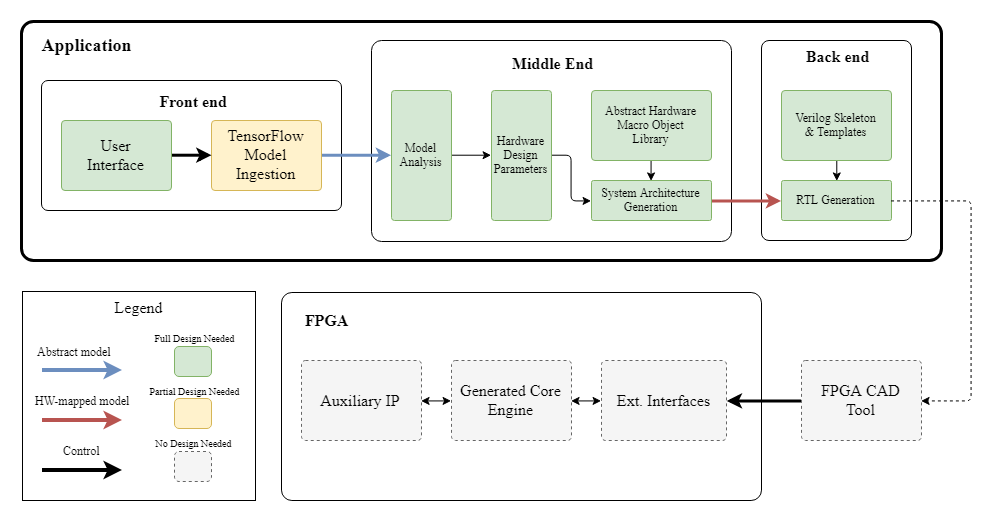
\includegraphics[width=\textwidth]{figures/system_block_diagram}
    \caption{System block diagram}\label{fig:system_block_diagram}
\end{figure}

\section{Project Specifications}

\subsection{Functional Specifications}

\begin{table}[H]
\centering
\caption{Functional specifications}\label{tab:func_specs}
\begin{tabularx}{\textwidth}{llX}
\toprule
Specification & Necessity & Description \\
\midrule
Hardware Functional Correctness & Essential & \gls{fpga} \gls{neural_net} inference behaviour must be identical to running the same optimized model on a CPU. \\
Synthesizable \gls{rtl} Output & Essential & \gls{rtl} generation must result in code synthesizable by industry-standard synthesizers. \\
Constraint Specification & Essential & The hardware resource constraints (i.e. logical element usage) needs to be obtained by the user interface. \\
Model Ingestion & Essential & The user-trained model must be successfully ingested into an intermediate data graph. \\
Model Analysis & Essential & Must accurately calculate user's model requirements for operations such as convolutions, adders, etc. \\
Model Compression & Essential & The compressed model must improve or maintain the model size on the \gls{fpga}. \\
\gls{fpga} space constraints & Essential & Compressed model must be able to fit on the available \gls{fpga} area as specified by the user. \\
Report of Optimization Metrics & Non-essential & Statistics such as \gls{fpga} area used and all optimizations made must be shown to the user so changes are transparent. \\
\bottomrule
\end{tabularx}
\end{table}

\subsection{Non-Functional Specifications}

\begin{table}[H]
\centering
\caption{Non-functional specifications}\label{tab:non-func_specs}
\begin{tabularx}{\textwidth}{llX}
\toprule
Specification & Necessity & Description \\
\midrule
Usability & Essential & User's interface with the program must be intuitive and easy to use. \\
Locally Executable & Essential & Must be able to be run on a local workstation with Linux support. \\
Process Runtime & Essential & The runtime of the system is less than 24 hours. \\
Practicality & Essential & Able to fit industry-standard \gls{neural_net} models. \\
Scalability & Non-essential & The architecture of the software allows for expansion the use of large models. \\
Power Usage & Non-essential & \gls{fpga} should consume less power than the CPU running the same neural net. \\
\bottomrule
\end{tabularx}
\end{table}

\section{Detailed Design}

The system is designed in three main sections: the front-end, middle-end, and back-end. The front-end interfaces with user configuration data and transforms the model and user requirements into intermediate forms used by other parts of the system. The middle-end of the system completes optimization at a model and at a hardware level. The model is first optimized to be transformed into hardware through model compression. Hardware generation then generates an intermediate hardware format that translates the model into hardware blocks. The back-end then takes this hardware format and outputs Verilog code that can be compiled by \gls{fpga} vendor tools in \gls{rtl} generation.

Since the initial application of this system is in an autonomous vehicle, the neural nets chosen for analysis are segmentation networks for object detection. Segmentation networks predict objects and segments them by pixel over an input image. DeepLab is one such example of this class of networks \cite{Chen2018DeepLab:-Semant}. DeepLab is state-of-the-art, highly accurate, and popular network that is being implemented for the task of dense object prediction tasks. This report uses the MobileNet variant of DeepLab for analysis.

\subsection{User Interface}

The input to the system is a configuration file which defines how the system operates. This includes configurations for the TensorFlow model and system parameters and goals. Each entry in the configuration file is a key-value pair that describes one property of the system.

The first section of the example configuration file shown in Listing \ref{lst:config_file} specifies various on-board resource utilization constraints. The maximum size of on-chip memory and maximum number of \glspl{le} that are available to the target \gls{fpga} for execution of a user model are defined by max\_mem\_bytes and max\_le\_count respectively. Resource utilization is an important factor to consider as different areas of the target \gls{fpga} may be used by different applications. The [APPLICATION] section defines the input and output of the system. The input\_model\_path points to the TensorFlow model to be deployed to the target \gls{fpga}. The configuration file is parsed using Python's native configparser library.

The input TensorFlow model is specified in Google's Protocol Buffer format which is a framework for serializing structured data. In addition to the TensorFlow model, the names of the input and output \glspl{tensor} are also supplied by the user. The input and output \glspl{tensor} are used in the TensorFlow Model Ingestion module to create our abstract model of the network.

\begin{figure}
\centering
\begin{lstlisting}[caption={Sample configuration file}, label=lst:config_file]
[FPGA]
fpga_family="intel"
max_mem_bytes=6000000
max_le_count=1150000

[APPLICATION]
input_tensor_name="input:0"
output_tensor_name="softmax:0"
input_model_path="/path/to/model_frozen.pb"

output_model_path="/path/to/out_model_frozen.pb"
\end{lstlisting}
\end{figure}

\subsection{TensorFlow Model Ingestion}

The model ingestion process involves reading and parsing a TensorFlow model specified in the Protocol Buffer format. During this process, TensorFlow API is used to perform the transformation of the text description of the model to a \gls{dag} representation of the same model \cite{Google-Inc.2018TensorFlow-API-}. The code snippet in Listing \ref{lst:parse_pb} demonstrates the usage of TensorFlow API to load and parse an existing model.

\begin{figure}
\centering
\begin{lstlisting}[caption={Sample code that parses a .pb file}, label=lst:parse_pb, language=Python]
def create_graph(self):
    # Creates graph from a saved .pb file
    with tf.gfile.FastGFile(self.modelPath, "rb") as f:
        graph_def = tf.GraphDef()
        graph_def.ParseFromString(f.read())
        _ = tf.import_graph_def(graph_def, name="")
        return graph_def
\end{lstlisting}
\end{figure}

\subsection{Model Compression}

One of the biggest challenge in deploying a \gls{neural_net} to an FPGA is the complexity of the model which often requires a huge amount of hardware resources. Studies have shown that quantization drastically reduces memory and hardware footprint while sacrificing inference accuracy \cite{Sheng2018A-Quantization-}. The quantization process in TensorFlow uses a uniform quantizer, in which the quantization steps are of equal size. The quantized value can be calculated as:
\begin{gather}
    x_\mathrm{quantized} = \left(\frac{x_\mathrm{float}}{\Delta x}\right) - \sigma_x \\
    \Delta x = \frac{x_\mathrm{max} - x_\mathrm{min}}{2^b - 1} \\
    \sigma_x = \frac{x_\mathrm{min}}{\Delta x}
\end{gather}
where $\Delta x$ represents the quantization step, b the bit width and $\sigma_x$ the offset value. $x_\mathrm{max}$ and $x_\mathrm{min}$ are the maximum and minimum values in floating point representation \cite{Sheng2018A-Quantization-}. The model quantization process involves traversing each node in the model graph obtained from the previous step in the pipeline and quantizing input and \gls{weight} values to 8-bit fixed point values. The model quantization process involves traversing each node in the model graph obtained from the previous step in the pipeline and quantizing the input and \gls{weight} values to 8-bit fixed point values.

TensorFlow provides a toolset under TensorFlow Lite containing tools for quantizing a fully trained inference model. The code snippet in Listing \ref{lst:optimize} shows the Google's TensorFlow Lite example provided for using graph transforms to quantize weights and strip unused nodes.

\begin{figure}
\centering
\begin{lstlisting}[caption={Code snippet to optimize a trained inference model}, label=lst:optimize, language=bash]
bazel build tensorflow/tools/graph_transforms:transform_graph
bazel-bin/tensorflow/tools/graph_transforms/transform_graph \
--in_graph=/tmp/frozen_inference_model.pb \
--outputs="softmax" --out_graph=/tmp/quantized_graph.pb \
--transforms='
add_default_attributes
strip_unused_nodes(type=float, shape="1,299,299,3")
remove_nodes(op=Identity, op=CheckNumerics)
fold_constants(ignore_errors=true)
fold_batch_norms fold_old_batch_norms
quantize_weights
quantize_nodes strip_unused_nodes sort_by_execution_order
'
\end{lstlisting}
\end{figure}

A more targeted pruning technique can be applied when considering the physical manifestation of the multiplications required within each convolution layer. The result of quantization of \gls{kernel} weights in convolution layers to an 8-bit fixed-point representation is that large portion of the \gls{cnn} parameters can be represented by zero, one or a power of two \cite{Abdelouahab2017Hardware-Automa}. This means that the physical hardware representing the multiplication can be removed or replaced with a wire or shift register. This intelligent design can reduce the resource utilization in the \gls{fpga} implementation. This can be especially efficient given that the multiplication with a set of weights in a quantized \gls{kernel} can be done in a loop over multiple cycles for a given set of input feature maps. This means that the physical hardware representing the multiplication can be removed or replaced with a wire or shift register. The final compressed model is converted back to a Protocol Buffer file and saved to the output path specified in the configuration file.

\subsection{Hardware Architecture Generation}

\subsubsection{Hardware Architecture}

The hardware architecture generation process performs the transformation of the graph representation of a \gls{neural_net} to an abstracted hardware design. This process must map the computations to a set of defined hardware blocks, while maintaining the sequence of operations and accuracy. That is, each computation that would have been performed on a CPU is identically performed on the \gls{fpga}.

Several broad classes of architectures were explored to determine a framework within which the hardware architecture is generated. An important requirement for the hardware architecture generation is that it maximizes the resource utilization and throughput, while minimizing the latency. It must also be able to fit a wide variety of \glspl{cnn}. Therefore, these metrics are used to select the class of architecture that would best meet the requirements.

\subsubsection{Direct Hardware Mapping}

\begin{figure}
    \centering
    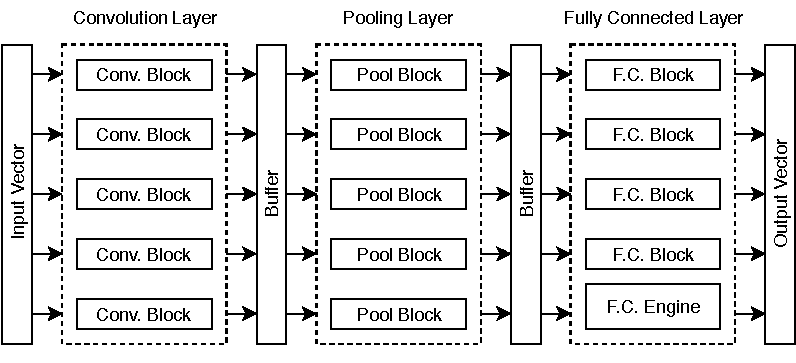
\includegraphics[width=\textwidth]{figures/direct_hardware_mapping}
    \caption{Direct hardware mapping \cite{Abdelouahab2017Hardware-Automa}}\label{fig:direct_hardware_mapping}
\end{figure}

The primary approach to mapping a \gls{neural_net} in hardware is to create dedicated hardware for each operation in the \gls{neural_net} evaluation. At the core of the \gls{cnn} is the convolution operation, where a two-dimensional matrix of weights (\gls{kernel}) sweeps across the entire input matrix, calculating the inner product of the kernels and the window over which it is convolving. Within the layer, each \gls{kernel} has a constant dimension. The kernels are learned in the training phase of the network.

A series of multipliers perform the multiplication between each of the matrix entries, followed by a series of adders which compute the sum of these products. This operation is referred to as a \gls{mac}. The dimensions of the inputs and outputs are well constrained within a layer, allowing the generation of \gls{rtl} modules by analyzing each layer.

Each \gls{kernel} of the convolutional network would be mapped directly to hardware based on its different \glspl{filter}. As an example, the first layer of AlexNet has 96 \glspl{filter} of size 11\times 11\times 3. Each \gls{filter} performs 3025 matrix multiplications over the input volume \cite{Krizhevsky2017ImageNet-Classi}. If every multiplication operation is performed by dedicated hardware, a total of 105,415,200 multipliers would be required, which severely exceeds the capabilities of any \gls{fpga}. Abdelouahab et al. have determined that approximately 70\% of multiplications in a \gls{cnn} could be reduced to a zero, pass-through, or shift operation \cite{Abdelouahab2017Hardware-Automa}. However, despite the reduction, a fully parallel mapping would still result in over 30 million multipliers, an order of magnitude greater than the 1.5 million logic elements available in a relatively large \gls{fpga} \cite{Intel-Corp.2018IntelR-ArriaR-1}.

Instead, each unique \gls{filter} receives dedicated hardware, and their matrix \gls{mac} operations are performed serially over the input volume. This results in a great reduction of the number of multipliers, to approximately 10,000 for the first layer of AlexNet. Thus, each layer of the \gls{neural_net} would map to a dedicated bank of logic that would perform its sequence of multiplications. Buffers are inserted between layers to resolve timing closure, creating a pipeline.

\subsubsection{Layer-Based Processing Banks}

\begin{figure}
    \centering
    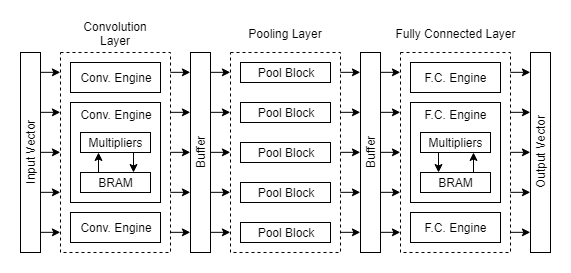
\includegraphics[width=\textwidth]{figures/layer-based_processing}
    \caption{Layer-based processing banks}\label{fig:layer-based_processing}
\end{figure}

In this architecture, the number of multipliers in a layer is greatly reduced. Each layer now contains a set of convolution engines, which would perform the \glspl{mac} of a subset of a layer's \glspl{filter} in parallel. This results in the \gls{filter} values needing to be stored and quickly accessed. The \gls{fpga} contains many banks of on-chip distributed \gls{sram} blocks, called \glspl{bram} which can be quickly accessed. The amount of memory resources vastly outnumbers the logic elements \cite{Intel-Corp.2018IntelR-ArriaR-1}. Thus, by using variable input multipliers and leveraging the on-chip memory, the number of multiplication resources can be reduced, allowing the fit of a larger network. However, latency and memory requirements increase. Furthermore, the memory resources now limit the size of the network which can be fit because the memory is shared between inter-layer results and \gls{filter} values.

\subsubsection{Layer-Scheduled Shared Multipliers}

\begin{figure}
    \centering
    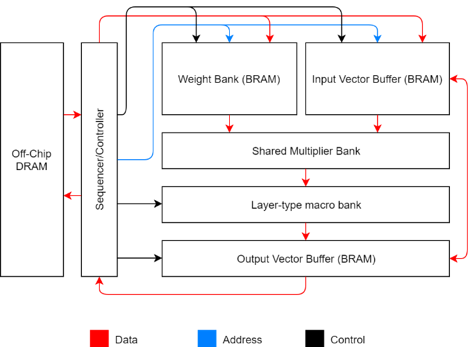
\includegraphics[width=\textwidth]{figures/layer-scheduled_multiplier}
    \caption{Layer-scheduled multiplier sharing \cite{Ma2017An-automatic-RT}}\label{fig:layer_scheduled_multiplier}
\end{figure}

A third architectural approach maximizes hardware reuse by implementing a shared multiplier bank between many layers. A central sequencer controls the memory addresses and execution order of each layer in the shared pipeline. Each different type of layer is mapped to a bank of resources which are reused every time the layer type is processed. The sequencer addresses the parameter memory and the input data memory to load the operands to the shared multiplier bank. The layer macro then processes the results of the multiplication based on the layer type \textemdash{} for instance, a convolution macro would contain a bank of adders and accumulators to sum the results of the multiplier bank. The results of the layer are then stored into the output data memory. When a layer has finished, the output memory is swapped with the input memory such that the next layer would use the results of the current layer, maximizing memory resource reutilization.

\subsubsection{Decision}

The specification for this tool requires a hardware architecture class with the highest resource efficiency. That is, given a fixed \gls{fpga}, being able to fit the largest network at a high throughput. A weighted decision matrix is used to determine the most efficient solution. Between the proposed architectural approaches, several criteria are used to determine the best approach, shown in the Table \ref{tab:hw_arch_criteria}.

\begin{table}
\centering
\caption{Hardware architecture class criteria}\label{tab:hw_arch_criteria}
\begin{tabular}{lcccc}
\toprule
       & Hardware Efficiency & Maximum Model Size & Throughput & Latency \\
\midrule
\Gls{weight} & 0.4 & 0.3 & 0.2 & 0.1 \\
\bottomrule
\end{tabular}
\end{table}

 Hardware efficiency is the ratio of used hardware to unused hardware in any given clock cycle. The maximum model size is quantified by the largest number of weights that can be stored using any given method on the \gls{fpga}, given no off-chip memory usage. These two factors determine whether the tool can implement practical \glspl{neural_net} given a fixed \gls{fpga} and are thus the higher weighted criteria.

The throughput is defined as the number of input vectors which can be processed in a clock cycle. The latency is the number of clock cycles between the input and output of the pipeline. These two metrics determine the usability of the network in a time-sensitive system. A theoretical estimate of the throughput and latency are used\textemdash{}the actual values are highly dependent on the \gls{cnn} model.

The hardware efficiency, throughput, and latency factors are calculated given several assumptions. Given that approximately 90\% of operations in a convolutional \gls{neural_net} are convolutions \cite{Cong2014Minimizing-Comp}, a hypothetical \gls{cnn} is used to provide simple calculations; it has three scaling convolutional layers, with each one being half the size of the previous one. The \gls{filter} size of every layer is 2\times 2\times 2, scaling each subsequent layer by a factor of $\frac{1}{2}$. The initial input layer is a 100\times 100\times 2 matrix. Furthermore, it is assumed that the network uses all the resources of a very small hypothetical \gls{fpga}. The maximum model size is calculated using the maximum resources available in an Arria 10 \gls{fpga}.

For the direct hardware map and layer-based processing banks, the hardware of the later stages may not be active in every cycle since it may take many cycles for the earlier layers to process their inputs. If the number of multipliers per layer are fixed, since every layer has a fixed number of kernels, the hardware efficiency $\eta$ of the direct hardware map model is calculated as follows:
\begin{equation}
    \eta = \frac{\sum_n \text{\# multipliers in layer} \times \frac{1 \text{ active cycle}}{4^n \text{ cycles}}}{\text{total multipliers}} = \frac{\frac{4}{1} + \frac{4}{4} + \frac{4}{16}}{16} = 0.33
\end{equation}
The hardware efficiency of the layer-based processing bank is calculated as follows:
\begin{equation}
    \eta = \frac{\sum_n \text{\# multipliers in layer} \times \frac{1 \text{ active cycle}}{4^n  \text{ cycles}} \times \frac{1}{2 \text{ cycles per input point}}}{\text{total multipliers}} = \frac{\frac{2}{1} + \frac{2}{8} + \frac{2}{32}}{6} = 0.39
\end{equation}

For the shared multiplier method, the number of multipliers is equal to the maximum number of multipliers need by any layer to process a single output point. Given that each layer has the same \gls{filter} dimension and \gls{filter} count, in this case every multiplier can be used in every cycle, with a decreasing number of cycles per layer due to the downscaling of layers. Thus, the efficiency of this system with this network is 1. However, in a real network, a portion of its hardware resources may be unused due to layers having different \gls{filter} counts and thus needing fewer multipliers. Through optimizations in the schedule, the unused multipliers and adders can be used to perform parallel calculations from the input vector, still allowing an efficiency of close to 1.

The maximum model size calculations assume that each parameter will be stored as an 8-bit byte. The maximum model size is limited by the \gls{le} count of the \gls{fpga} for the direct hardware mapping method. Based on academic research, a 60000-parameter network uses 50452 \glspl{le} in a direct map, using 5-bit representation \cite{Abdelouahab2017Hardware-Automa}. The following equation determines the parameter count $P$ using the Arria 10 \gls{fpga} \cite{Intel-Corp.2018IntelR-ArriaR-1} used for this project's metrics:
\begin{equation}
    P = \frac{\text{\# LEs}}{\text{\# LEs/param}} = \frac{1577000}{\frac{50452}{60000 \times 5 \text{ bits}} \times 8 \text{bits}} = 1.17 \times 10^6
\end{equation}

For the layer-based processing banks, the \gls{le} count is constrained by the \gls{bram} available on the chip. In this architecture, a part of the \gls{bram} needs to be used to buffer intermediate results of subsequent layer. Typically, parameter count increases with layer count and layer dimensions. It is not possible to define a function of parameter count to buffer size, since each \gls{neural_net} architecture is vastly different. To arrive at an estimate, two \gls{cnn} types are examined; AlexNet, a shallow \gls{cnn}, has 60M parameters and 650000 inter-layer values; MobileNet, a deep \gls{cnn}, has 1.7M parameters, and 7M inter-layer values. New networks, especially for image segmentation, tend to be deeper rather than wider \cite{Howard2017MobileNets:-Eff}. Thus, it is estimated that the parameters are allocated $\frac{1}{6}$ of the \gls{bram} resources.
\begin{equation}
    P = \frac{\text{BRAM bytes}}{6} = \frac{6750000 \text{ bytes}}{6} = 1.1 \times 10^7
\end{equation}

The shared multiplier approach stores the inputs and outputs to one layer in any given cycle. Therefore, the most \gls{bram} needed for intermediate value storage is twice the size of the largest layer. In MobileNet, the largest layer requires 1.2MB of buffers \cite{Howard2017MobileNets:-Eff}. Thus, the number of parameters which can be stored is:
\begin{equation}
    P = 6750000 \text{ bytes} - 2 \times 1200000 \text{ bytes} = 4.35 \times 10^7
\end{equation}

Given that the same \gls{cnn} is used, and that each architecture is resource-saturated by parameters\textemdash{}that is, fitting the same network in the smallest \gls{fpga} that each architecture allows\textemdash{}a relative ranking of throughput and latency is estimated.

The throughput metric is defined by the number of input matrices the architecture can process per unit time. The direct hardware mapping approach can process a matrix the fastest, because it has a dedicated multiplier for each individual parameter. The layer-based processing banks has a lower throughput because its resource sharing results in the next layer needing to be stalled when the \gls{fpga} resources are saturated. Finally, the shared multiplier bank has the lowest throughput under saturation\textemdash{}every layer must wait for the previous layer to be completed.

A direct hardware map is again able to finish an image in fewer cycles than the other two approaches. The layer-based processing bank requires more cycles to loop over its parameter bank. Finally, the shared multiplier bank has the longest latency.

The weighted decision matrix in Table \ref{tab:decision_matrix} compiles and normalizes the scores for each architecture. Based on this analysis, the shared-multiplier method is the most effective approach for generating hardware. It maximizes hardware resource usage and the model size, making the \gls{rtl} generator most compatible with the most networks, especially new, deep networks with large parameter counts. While the direct hardware mapping method is potentially very fast, it still requires a vast amount of resources that severely limits the size of the \gls{neural_net} that can be implemented.

\begin{table}
\centering
\caption{Normalized weighted decision matrix}\label{tab:decision_matrix}
\begin{tabular}{lccccc}
\toprule
& HW Efficiency & Max Model Size & Throughput & Latency & \textbf{Total} \\
\midrule
\Gls{weight}            & 0.4           & 0.3            & 0.2        & 0.1     & \textbf{1.0} \\
Direct Map        & 3.3           & 0.3            & 10         & 10      & \textbf{4.4} \\
Layer-Multiplier  & 3.9           & 2.5            & 5          & 5       & \textbf{3.8} \\
Shared-Multiplier & 10            & 10             & 1          & 1       & \textbf{7.3} \\
\bottomrule
\end{tabular}
\end{table}

The ability for this architecture to maximally reuse on-chip \gls{dram} allows larger models to be processed. The throughput of the system can be further improved by optimizing the scheduling and pipelining the logic to allow the \gls{fpga} to run at a faster clock.  Therefore, this architecture is the best approach for the \gls{rtl} generation tool, giving the most flexibility and practicality in the \glspl{neural_net} that can be used.

\subsection{Model Analysis}

\subsubsection{Model Representation}

The model analysis will be primarily supported by the API provided by TensorFlow's GraphDef class. A GraphDef structure is created from the ProtoBuf library and is Google's a convenient representation of the \gls{neural_net} structure. A trained inference model can be stored as a GraphDef ProtoBuf file with all its weights using the ``freezing'' feature provided by TensorFlow. This allows a standalone ProtoBuf file to contain all information required to restore and run the model. GraphDef can be saved as either a binary\textemdash{}used for large models\textemdash{}or a human readable text file.

Once passed, the GraphDef object can be traversed by moving through each of the nodes \cite{Google-Inc.2018A-Tool-Develope}. NodeDef object in the graph contains name, op, input, device, and attr specifications. The two key specifications of significance in this application are the operation (op) and attribute (attr). The operation specifies the TensorFlow operation for the node (ex. Convolution, \gls{relu}, etc.), this can be used to identify the operation when traversing through the graph. Each convolution node takes as input a constant input\textemdash{}containing the input feature map, and the constant weights matrix.

\subsubsection{Footprint Estimation}

The footprint estimator provides an approximate count of \glspl{mac} required to execute a GraphDef model. Studies have shown that convolutions take up to 90\% computation and runtime in a deep \gls{cnn} \cite{Wang2017Data-centric-co}. Due to the computation intensive nature of convolutions, only operations that involve convolutions or operations that are associated with convolutions are analyzed in the footprint estimator. The set of included operations are: Conv2D, Depthwise\_Conv2D, ReLu, MaxPool, SoftMax and Fully\_Connected. The number of \glspl{mac} require for each operation are specified in Table \ref{tab:macs_required}. $C$, $H$, and $W$ denote respectively channel count, height, and width.

\begin{table}
\centering
\caption{Equations for calculating the number of \glspl{mac} required}\label{tab:macs_required}
\begin{tabular}{ll}
\toprule
Operation        & Equation \\
\midrule
Conv2D           & $C_\mathrm{in} \times C_\mathrm{out} \times H_\mathrm{out} \times W_\mathrm{out} \times H_\mathrm{kernel} \times W_\mathrm{kernel}$ \\
Depthwise Conv2D & $H_\mathrm{kernel} \times W_\mathrm{kernel} \times C_\mathrm{in}$ \\
ReLu             & $H_\mathrm{out} \times W_\mathrm{out} \times C_\mathrm{out}$ \\
MaxPool          & $H_\mathrm{in} \times W_\mathrm{in} \times C_\mathrm{in}$ \\
SoftMax          & $H_\mathrm{in} \times W_\mathrm{in} \times C_\mathrm{in}$ \\
Fully Connected  & $C_\mathrm{in} \times C_\mathrm{out} \times H_\mathrm{out} \times W_\mathrm{out} \times H_\mathrm{in} \times W_\mathrm{in}$ \\
\bottomrule
\end{tabular}
\end{table}

\subsubsection{Scheduler}\label{sec:scheduler}

The scheduler takes as input the GraphDef and any user constraints to output a set of instructions, a set of weights and the inputs to be loaded into on-chip memory. The instructions will be fetched by the sequencer and the instructions will then specify the set of weights and lines of input to load into the macro (multipliers, adders, accumulator blocks, \gls{relu}, etc.). The instruction set will also specify the amount of clock-cycles required for processing for each layer as determined by the scheduler.

To generate the instruction-set, the scheduler optimizes on the user constraints: execution speed (in frames per second), \gls{fpga} \gls{le} count and memory usage. A significant amount of resources and computational latency is spent on the convolutional layers in a \gls{cnn}. Convolutions involve three dimensional \gls{mac} of input features with a set of \gls{kernel} weights. We use the framework established in \cite{Ma2017Optimizing-Loop} to break down convolutions into four separate loops as shown in Figure \ref{fig:four_loops}.

\begin{figure}
\centering
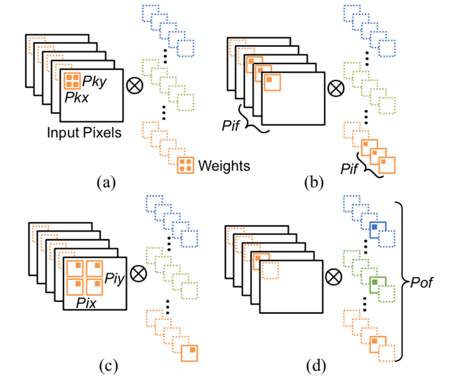
\includegraphics{figures/four_loops}
\caption{The four loops involved in a convolution operation \cite{Ma2017Optimizing-Loop}}\label{fig:four_loops}
\end{figure}

Given the user constraints, the controller chooses the parameters for three operations: loop unrolling, loop tiling and loop interchange. For this particular project, loop tiling and loop interchange will not be used, instead all efforts will be focused on optimizing the loop unrolling. The dimensions of the \gls{kernel} window are specified by (Nkx, Nky), while (Nix, Niy) and (Nox, Noy) specify the dimensions of one input and output feature map, respectively. Each of the loops can then be denoted as shown in Table \ref{tab:loop_vars}.

\begin{table}[hbp]
\centering
\caption{Detailed representation of variables denoting each loop in a convolution \cite{Ma2017Optimizing-Loop}}\label{tab:loop_vars}
\begin{tabular}{l cc cc cc c c}
\toprule
& \multicolumn{2}{c}{\Gls{kernel} dims} & \multicolumn{2}{c}{Input dims} & \multicolumn{2}{c}{Output dims} & \multicolumn{2}{c}{\# of input/output channels} \\
\midrule
Loop designator & \multicolumn{2}{c}{Loop 1} & \multicolumn{2}{c}{Loop 3} & \multicolumn{2}{c}{Loop 3} & Loop 2 & Loop 4 \\
Convolution dims & $N_\mathrm{kx}$ & $N_\mathrm{ky}$ & $N_\mathrm{ix}$ & $N_\mathrm{iy}$ & $N_\mathrm{ox}$ & $N_\mathrm{oy}$ & $N_\mathrm{if}$ & $N_\mathrm{of}$ \\
Loop tiling & $T_\mathrm{kx}$ & $T_\mathrm{ky}$ & $T_\mathrm{ix}$ & $T_\mathrm{iy}$ & $T_\mathrm{ox}$ & $T_\mathrm{oy}$ & $T_\mathrm{if}$ & $T_\mathrm{of}$ \\
Loop unrolling & $P_\mathrm{kx}$ & $P_\mathrm{ky}$ & $P_\mathrm{ix}$ & $P_\mathrm{iy}$ & $P_\mathrm{ox}$ & $P_\mathrm{oy}$ & $P_\mathrm{if}$ & $P_\mathrm{of}$ \\
\bottomrule
\end{tabular}
\end{table}

Loop unrolling can be done for any one of the four loops, each option changing resource reusability as well as memory access patterns. The per cycle operations required for each method are summarized below. Table \ref{tab:unrolling} shows their associated memory accesses, resources and computations in each cycle.

\paragraph{Loop 1 unrolled}
Inner product of all weights in a $P_\mathrm{kx} \times P_\mathrm{ky}$ \gls{kernel} and inputs for each $(x_k, y_k)$ for a single layer
\paragraph{Loop 2 unrolled}
The $P_\mathrm{kx} \times P_\mathrm{ky}$ \gls{kernel} is evaluated at a single $(x_k, y_k)$ for all $P_\mathrm{if}$ layers
\paragraph{Loop 3 unrolled}
$P_\mathrm{kx} \times P_\mathrm{ky}$ \gls{kernel} is evaluated at a single $(x_k, y_k)$ for all $(x, y)$ in $P_\mathrm{ix} \times P_\mathrm{iy}$ of a single layer
\paragraph{Loop 4 unrolled}
A single input pixel is evaluated on $P_\mathrm{of}$  different $P_\mathrm{kx} \times P_\mathrm{ky}$ \glspl{kernel} at a fixed position $(x_k, y_k)$

\begin{table}[hbp]
\centering
\caption{Memory access and resource utilization for unrolling convolution loops}\label{tab:unrolling}
\begin{tabular}{ll llll}
\toprule
            && Loop 1 unrolled & Loop 2 unrolled & Loop 3 unrolled & Loop 4 unrolled \\
\midrule
\multicolumn{6}{l}{Memory access} \\
& Weights & $P_\mathrm{kx} \times P_\mathrm{ky}$ & $P_\mathrm{if}$ & 1 & $P_\mathrm{of}$ \\
& Input pixels & $P_\mathrm{kx} \times P_\mathrm{ky}$ & $P_\mathrm{if}$ & $P_\mathrm{ix} \times P_\mathrm{iy}$ & 1 \\
\multicolumn{6}{l}{Resources} \\
& Fan-in adder tree & $P_\mathrm{kx} \times P_\mathrm{ky}$ & $P_\mathrm{if}$ & 0 & 0 \\
& Multipliers & $P_\mathrm{kx} \times P_\mathrm{ky}$ & $P_\mathrm{if}$ & $P_\mathrm{ix} \times P_\mathrm{iy}$ & $P_\mathrm{of}$ \\
& Accumulators & 1 & 1 & $P_\mathrm{ix} \times P_\mathrm{iy}$ & $P_\mathrm{of}$ \\
\bottomrule
\end{tabular}
\end{table}

From Table \ref{tab:unrolling}, a set of variables to be used by the optimization algorithm can be derived:
\begin{gather}
\text{Multipliers Per Cycle} = P_\mathrm{kx} \times  P_\mathrm{ky} \times  P_\mathrm{ix} \times  P_\mathrm{iy} \times P_\mathrm{if} \times  P_\mathrm{of} \\
\text{Distinct Weights per Cycle} = P_\mathrm{kx} \times  P_\mathrm{ky} \times  P_\mathrm{if} \times  P_\mathrm{of} \\
\text{Distinct Pixels per Cycle} = P_\mathrm{if} \times (( P_\mathrm{ix} - 1)S + P_\mathrm{kx}) \times (( P_\mathrm{iy} - 1)S + P_\mathrm{ky}) \\
\begin{aligned}
    \text{Weight Reuse} &= \frac{\text{Multipliers Per Cycle}}{\text{Distinct Weights Per Cycle}} \\
                        &=  P_\mathrm{kx} \times  P_\mathrm{ky}
\end{aligned} \\
\text{Pixel Reuse} = \frac{\text{Multipliers Per Cycle}}{\text{Distinct Pixels Per Cycle}}
\end{gather}
With these, the read memory accesses for input pixels and weights can be calculated:
\begin{gather}
    \text{\# Weight Reads} = \frac{\text{Multipliers Per Cycle}}{\text{Weight Reuse}} \\
    \text{\# Pixel Reads} = \frac{\text{Multipliers Per Cycle}}{\text{Pixel Reuse}}
\end{gather}

For each layer, the scheduler generates the \gls{kernel} size $K$, feature dimension $(X, Y)$ and the number of iterations $\frac{N_\mathrm{of}}{P_\mathrm{of}}$. These correspond to the iteration over layers 1, 3 and 4, respectively. The sequencer uses the parameter in the following equation:
\begin{equation}
    k_x + k_y \times (X_i + 2 \times \text{PAD}) + \text{STRIDE} \times x \times \text{STRIDE} \times y \times (X_i + 2 \times \text{PAD})
\end{equation}
Where the PAD represents the zero padding and STRIDE represents the stride length of the \gls{kernel}. $k_y$ is generated by an internal counter in the sequencer that increases by 1 when $k_x$ equals $K - 1$. $x$ and $y$ iterate from 0 to $X_i - 1$ and $Y_i - 1$ respectively. The write address, similarly, iterates from 0 to $X_i \times Y_i$ \cite{Ma2017Optimizing-Loop}.

\subsection{Top Level Hardware System Framework}\label{sec:top_level_framework}

Figure \ref{fig:top_level} shows an example of a hardware system that can be generated, in this case based on MobileNet V2 \cite{Howard2017MobileNets:-Eff}. The framework of the hardware architecture remains fixed regardless of the \gls{neural_net} model. In Section 3, layer-scheduled multiplier sharing was the hardware framework selected for the generated system. % TODO

\begin{figure}
\centering
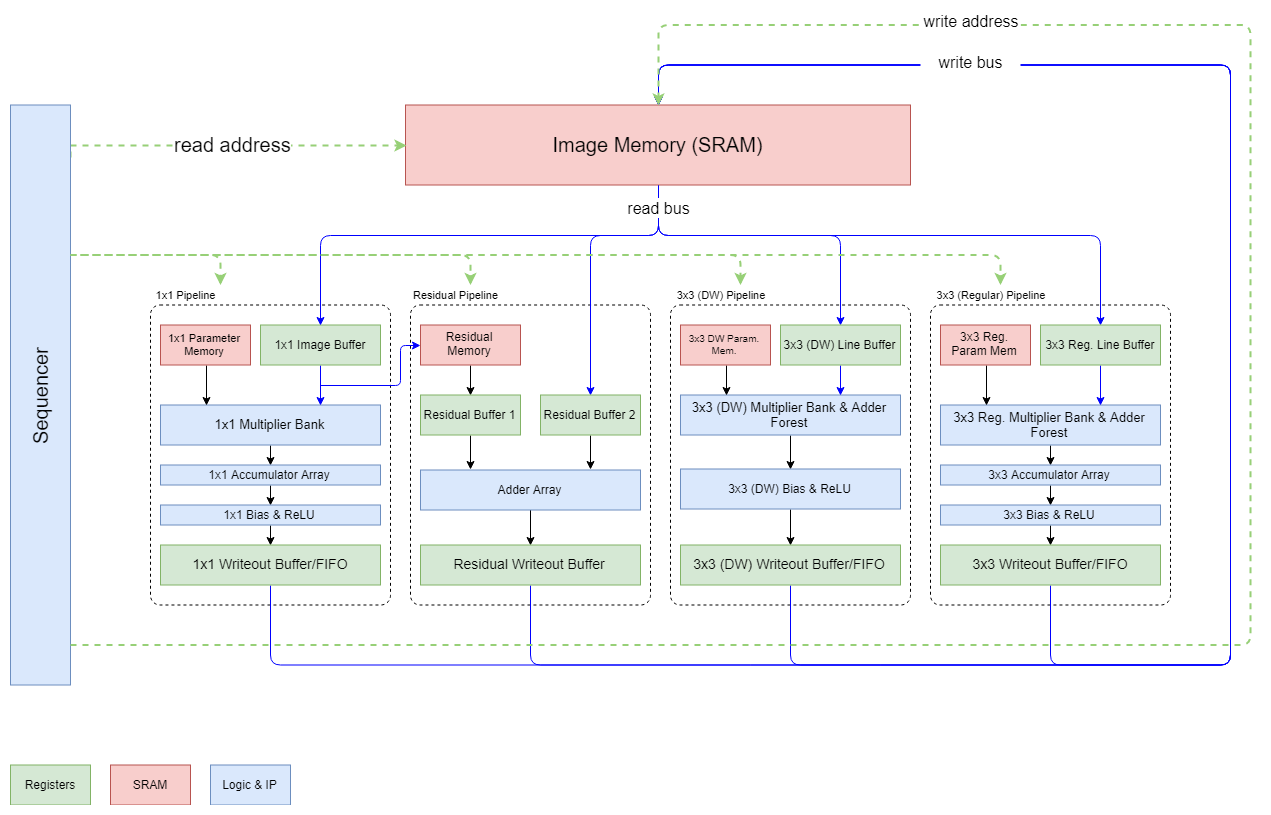
\includegraphics[width=\textwidth]{figures/top_level}
\caption{Hardware system top level framework}\label{fig:top_level}
\end{figure}

In practice, however, it is very expensive to implement data multiplexing for a large bank of multipliers, so the multiplier bank is split to accommodate for each layer type. Within each layer type, the dataflow from the memory to the multiplier bank and from the multiplier back to the memory must be consistent to remove the need for multiplexing, allowing faster operating hardware and simpler implementation at the cost of instantaneous hardware utilization. Convolution layers with identical \gls{kernel} dimensions can share processing pipelines, but different layers with different \gls{kernel} dimensions have different dataflow, and therefore are not able to share the same pipeline. Parameter memory is distributed to each of the separate processing pipelines so that it can be placed close to the logic that it will feed.

Figure \ref{fig:sequencer} shows a functional diagram of the operation sequencer block. The sequencer provides data flow control; it controls the addresses of the memories to provide the correct inputs to the multiplier bank; it also issues control signals for each layer-type macro. The sequencer reads a \gls{rom} storing microcode which describes the layer type and the loop parameters of each layer. This microcode is generated by a scheduler in model analysis. A fixed state machine within the sequencer uses the layer and loop parameters to generate the data and parameter memory addresses and to issue control signals for the macro blocks.

\begin{figure}
\centering
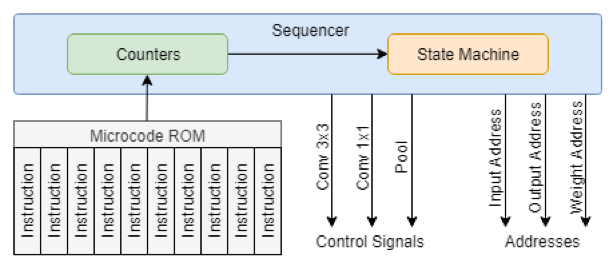
\includegraphics[width=0.7\textwidth]{figures/sequencer}
\caption{Operation sequencer}\label{fig:sequencer}
\end{figure}

To support segmentation networks, additional forms of convolution will be supported through sequencing. Atrous convolutions, commonly used in segmentation networks, have \glspl{conv_window} which skip adjacent values in the input volume \cite{Chen2018DeepLab:-Semant}. The sequencer would change its \gls{ram} addressing mode to skip consecutive addresses to create the dilated \gls{conv_window}.

\glspl{fpga} typically contain distributed \gls{sram} arrays, called \glspl{bram}. In Intel \glspl{fpga}, the most common type of \gls{bram} cell is a \SI{20}{\kilo\bit} array referred to as a M20K cell. The control interface for \glspl{bram} are variable, allowing them to be instantiated with a variety of widths and depths. Several arrays can be combined by the vendor synthesizer tool to create a larger array. With this in mind, the tool is able to flexibly define the dimensions of the buffers in \gls{rtl} generation to best suit the \gls{neural_net}.

The system architecture contains one large \gls{bram} array for storing layer weights, and one for storing inter-layer results. When one layer finishes its operations, the next layer uses its output as its input and stores its results in its previous layer's input area.

\subsection{Macro Generation}\label{sec:macro_gen}

A dedicated macro block is generated from a library of templates to process each type of layer (convolution, pooling, etc.) in the \gls{neural_net}. For layers of the same type, the same processing architecture is reused, with the scheduler coordinating different loop parameters using its microcode instructions. Convolution layers with different \gls{kernel} dimensions needs macro blocks which have different parameters but retain the same general architecture. The \gls{rtl} templates are highly parameterized so that their dimensions can be defined when they are instantiated.

Each macro block is controlled by the sequencer to loop over the input matrix using instructions written in microcode. The required macro blocks for a layer type and their design parameters are generated using the formulas outlined in the model analysis section.

The convolution macro contains buffers to enable data reuse in the convolution operation, adders and accumulators to sums the results of multiplications, and \gls{relu} modules. Cascading adders sum the results of the multiplication and \gls{bias} parameters. The precise format of the adder tree will vary based on degree of loop unrolling, \gls{filter} dimensions and different types of convolutions. In some cases, the additions may need to be split over multiple multiplication cycles, and therefore accumulators are required to sum each consecutive result. The \gls{relu} operation adds nonlinearity to \gls{neural_net} activations and exists as the final operation of a \gls{neural_net} layer. Following the \gls{relu} operation, the results are stored in a final output register bank to be written to memory.

Depth-wise convolutions are an example of a convolution layer which could have a different adder tree format. Depth-wise convolutions are commonly used in segmentation networks \cite{Howard2017MobileNets:-Eff}. They specify a single \gls{kernel} for every input layer, and each \gls{kernel} only convolves over that layer. Thus, the adder tree of a depth-wise convolution layer may be several parallel trees, each contributing to a single output value, with no accumulation over the input layers. This allows a high degree of parallelism while processing depth-wise convolution layers. However, this makes the depth-wise convolution pipeline incompatible with regular convolution pipelines, which requires accumulation across the input layers.

Every type of macro will be pipelined to maximize clock frequency. Each functional block of the macro block will be divided by a pipeline stage, as shown in Figure \ref{fig:convolution_macro} with the brackets to the right. To generally maximize data reuse and parallelism where resources are available, several \glspl{kernel} can be loaded to several parallel multiplier banks, adders, and accumulators (collectively named a `processing thread') using the same input data. This results in some arbitration required at the output bus by the schedule to avoid conflicts in result write out. There is usually a long latency before the next batch of outputs need to be written out while the next layer is being processed, allowing each of the separate processing threads to write out sequentially. Since the bulk of the processing is done in parallel, this method allows increased parallelism where hardware resources are available.

\begin{figure}
\centering
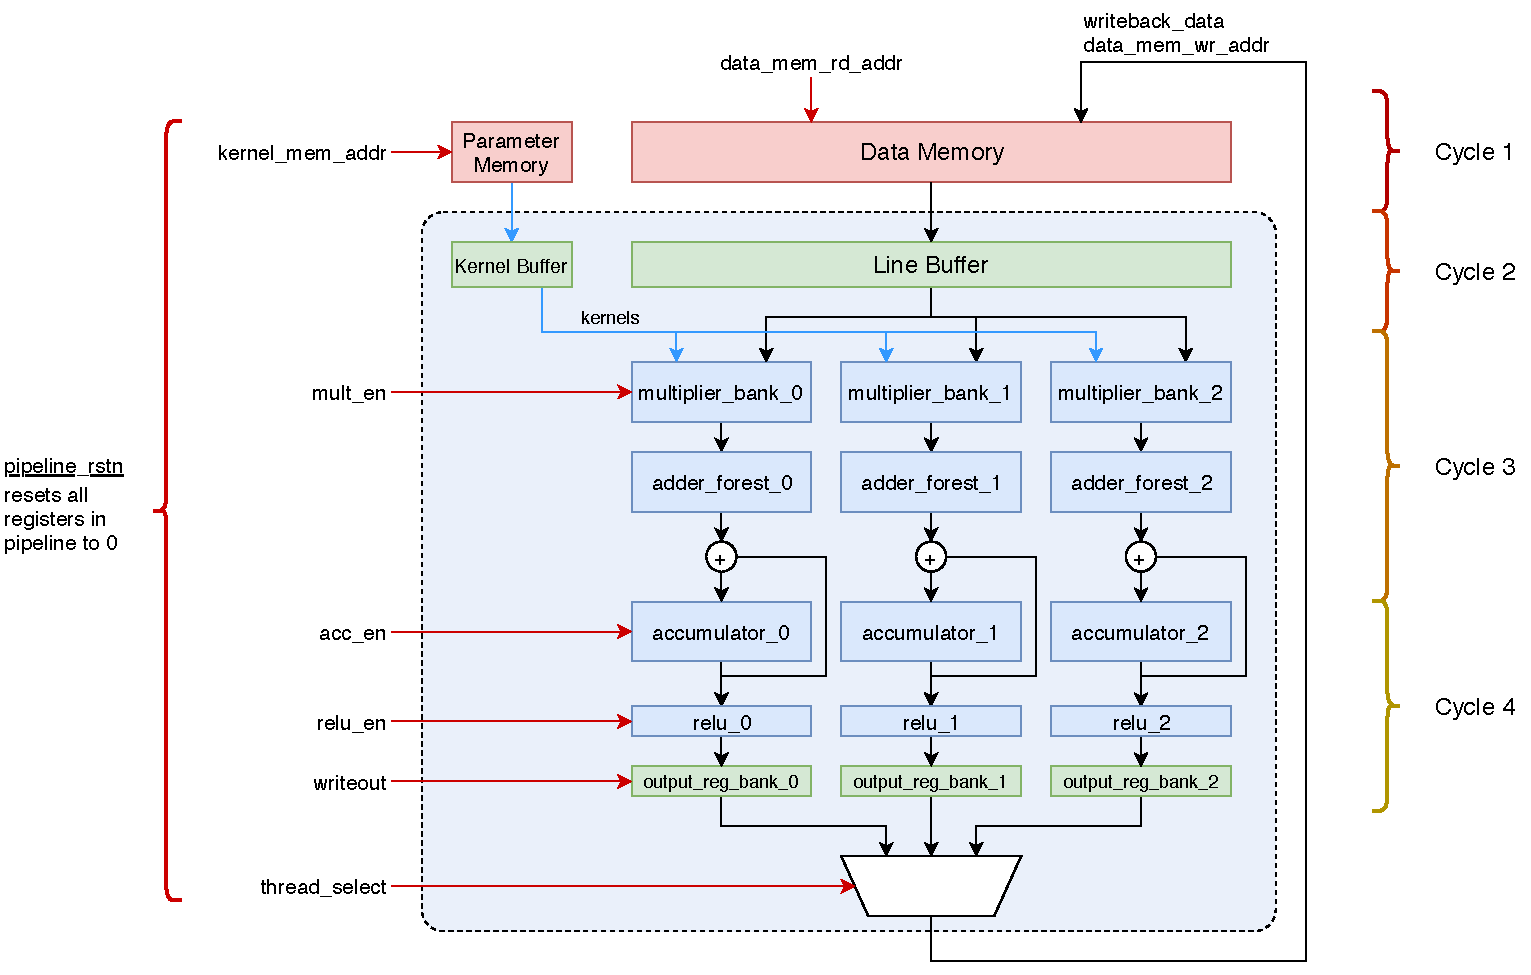
\includegraphics[width=\textwidth]{figures/convolution_macro}
\caption{Convolution macro block \cite{Ma2017An-automatic-RT}}\label{fig:convolution_macro}
\end{figure}

Modern convolutional \glspl{neural_net} often contain residual blocks (Howard, et al., 2017). Residual blocks add a connection between two layers of the same dimensions, summing the input of the first layer to the output of the second layer. To accommodate for this operation, a macro block containing a memory for temporarily storing the inputs to the first layer when it is being processed, and then adding the results of the second layer after it has been processed, is created. The residual pipeline is a simple adder array which adds two equal dimension arrays. The pipeline is similarly parameterized, and the parameters are generated during model analysis. It is controlled by the sequencer using dedicated microcode for flagging residual layers.

\begin{figure}
\centering
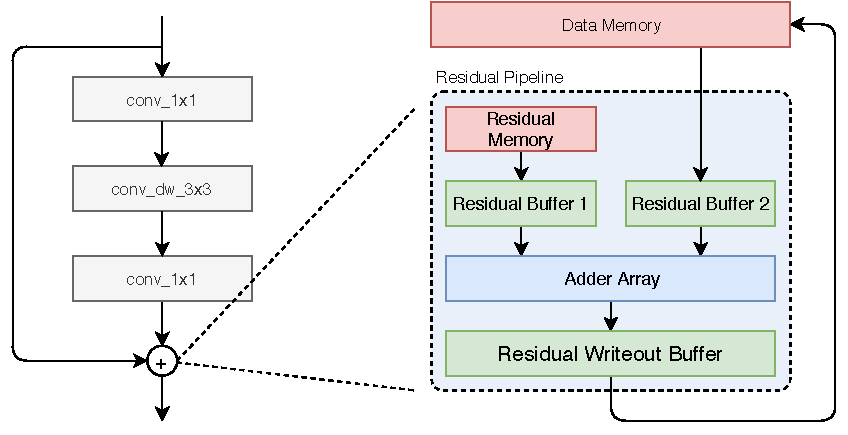
\includegraphics[width=\textwidth]{figures/residual_addition}
\caption{Residual addition}\label{fig:residual_addition}
\end{figure}

Some \glspl{neural_net} contain pooling operations. A pooling macro down samples the input volume by either taking the maximum or average of a window of the input volume and outputting it to an output volume. Depending on the type of pooling layers, a pooling macro may contain a bank of comparators to select the maximum value, or an accumulated divider to average the input values.

\begin{figure}
\centering
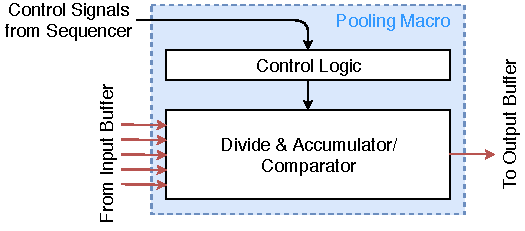
\includegraphics[width=\textwidth]{figures/pooling_macro}
\caption{Pooling macro block \cite{Ma2017An-automatic-RT}}\label{fig:pooling_macro}
\end{figure}

The multiplier bank must support the largest number required for a given layer and unrolling scheme in the network. Since multiplication hardware implemented using \glspl{le} are expensive, \glspl{fpga} typically include dedicated multiplication hardware in the form of hardened multipliers and DSPs \cite{Intel-Corp.2018IntelR-ArriaR-1}. Therefore, the multiplier bank will primarily be synthesized as hardened multipliers and DSPs using \gls{rtl} directives. \Glspl{le} will be used only when hardened resources are saturated.

\subsection{RTL Generation}\label{sec:rtl_gen}

The \gls{rtl} generation block transforms the \gls{dag} that represents the execution schedule and thus the list of hardware to a synthesizable \gls{rtl} codebase. A library of \gls{rtl} templates for each block of the system architecture is generated. The templates will be processed, and variable placeholders will be replaced by the parameters. An example of a Verilog module declaration template is shown in Listing \ref{lst:verilog_template}.

\begin{figure}
\centering
\begin{lstlisting}[caption={Verilog template}, label=lst:verilog_template, language=Verilog]
module adder_tree (
    /*AUTOINPUT*/
    input[7:0]      in0,                // adder inputs
    input[7:0]      in1,                // adder inputs
    input[7:0]      in2,                // adder inputs
    ...
    /*END AUTOINPUT*/

    // outputs
    output[7:0]     result              // result output
);
\end{lstlisting}
\end{figure}

The comments surrounding the input port will be parsed and the template will be expanded to the number of multiplication results for this adder tree module. Inherently, Verilog does not allow the generation of ports. This method allows for flexible generation of modules depending on the requirements set by model analysis. The generated Verilog is compatible with only Intel \glspl{fpga} as Intel \gls{ip} is used in part of the system architecture.

\subsection{Vehicle Integration}

While our project is application agnostic, the initial use case will be for an autonomous vehicle. The specific implementation of a vehicle interface is not within the scope of this project, but it is helpful to give some perspective on how the \gls{fpga} will communicate with the vehicle's driving and perception systems. The team at WATO will be implementing a \gls{pcie} driver that can speak to the \gls{fpga} board in the vehicle. This driver will contain a \gls{ros} adapter that can retrieve camera images to send to the \gls{fpga} and can also write the results after the \gls{fpga} processes the image. This will be tightly integrated with the remainder of the \gls{ros}-based WATO system.


\section{Prototype Data}

\subsection{System Functional Model}

The functional model for this system is a pure software component that is mainly designed for hardware verification purposes. Each hardware component is mapped to a software component, implemented in Python, of the functional model. The strong correlation between software and hardware components enables the functional model to accurately simulate hardware execution. In addition to having a one-to-one mapping, each component in the functional model is written in a specific way that follows a set of rules to closely mimic hardware behaviours. The set of rules are as follows:
\begin{enumerate}
    \item Registers are represented by variables
    \item Allowed operations on registers are assignment of constant and addition of constant or another register
    \item Comparisons should be only be tested against zero or constant
    \item For-loops should be converted to while-loops
    \item Divisions are not allowed
\end{enumerate}

On a high level, any convolutional \glspl{neural_net} can be considered as a series of convolutions.  Each convolutional layer in the model consists of a sequence of operations. The various operations involved can be generalized to load, store, add, multiply, \gls{relu} and accumulate. The functional model simulates hardware execution by creating a component for each operation involved in convolution. The load operation fetches input and weights from their respective memory bank and feed them into \gls{mac} blocks to perform convolution. Store writes the intermediate result of a \gls{mac} to output memory bank which will be accumulated across output \glspl{filter}. Add and multiply operations are the building blocks that represent adders and \glspl{mac} in hardware. Listing \ref{lst:databank_init} contains a code snippet that initializes the databank of the functional model. Input \glspl{tensor}, translated from Tensorflow, of shape 4D is reshaped into a 2D array. The databank is constructed as a two-dimensional array to match the physical layout of embedded memory on the \gls{fpga}. This allows the functional model to use the same memory addressing scheme as hardware.

\begin{figure}
\centering
\begin{lstlisting}[caption={Databank initialization in software}, label=lst:databank_init, language=Python]
def init_databank(self, preloaded_bank=None):
    if preloaded_bank is not None:
        self.databank = preloaded_bank
        self.write_hex_file(self.databank, 'data_bank.old')
        return

    # This is only valid for one model layer. x,y, and m will change
    # from layer to layer
    input_bytes = mdl.input_m * mdl.input_x * mdl.input_y
    output_bytes = mdl.kernel_count * mdl.input_x * mdl.input_y

    # Build the input data bank
    input_pixels = np.ones(input_bytes, dtype='float32')
    output_pixels = np.zeros(output_bytes, dtype='float32')

    concat_array = np.concatenate([input_pixels, output_pixels])
    self.databank = np.reshape(concat_array, [-1, mdl.databus_size])
\end{lstlisting}
\end{figure}

In addition to simulating hardware operations, the functional model is also responsible for opcode generation. An opcode is an instruction that contains various operating parameters that are essential in hardware execution. The general structure of an opcode is illustrated in Listing \ref{lst:opcode}.

\begin{figure}
\centering
\begin{lstlisting}[caption={General opcode format}, label=lst:opcode]
opcode {
    type (2 bits) // 01 = 1x1, 10 = 3x3 depthwise, 11 = 3x3 regular
    input_base (8 bits)
    output_base (8 bits)
    kernel_base (8 bits)
    kernel_count (8 bits)
    tiles_per_layer (8 bits)
    input_m (8 bits) // number of input channels
}
\end{lstlisting}
\end{figure}

The most important fields in an opcode are the base counters. The hardware relies on these counters to load input data and weights at the appropriate offsets to account for the shifting of \gls{kernel} window. The opcode generated by the function model can be directly used in hardware without further processing because the memory banks in the functional model are arranged in the exact same way memory banks are arranged in hardware. Listing \ref{lst:1x1_sim} shows the simulation of a 1x1 convolution operation using techniques, such as loop unrolling, described in earlier sections.

\begin{figure}
\centering
\begin{lstlisting}[caption={Simulation of 1x1 convolution in functional model}, label=lst:1x1_sim, language=Python]
def simulate(self, input_base, output_base, kernel_base, kernel_count,
             tiles_per_layer, input_m):
    # opcode generation
    class accumulator:
        # Implementation not shown
    class one_by_one_registers:
        # Implementation not shown

    # Generate the stateful accumulator hardware
    acc = accumulator(mdl.databus_size)
    r = one_by_one_registers()
    r.kernel = 0
    r.output_addr_kernel = 0
    r.kernel_addr_kernel = 0
    while r.kernel != kernel_count:
        r.tile = 0
        while r.tile != tiles_per_layer:
            r.data_addr_layer = 0
            r.layer = 0
            while r.layer != input_m:
                data, weight, bias = self.load(r.get_data_addr(),
                                               r.get_kernel_addr())
                res = self.multiply(data, weight)
                acc.add(res)
                # Counters for layer
                r.data_addr_layer += tiles_per_layer
                r.layer += 1
            r.tile += 1
            # Bias and ReLu
            # print(acc.accumulator, bias)
            bias_out = self.add(acc.accumulator, bias)
            relu_out = self.relu(bias_out)
            self.store(r.get_output_addr(), relu_out)
            acc.reset()
        #Counter for kernel
        r.output_addr_kernel += tiles_per_layer
        r.kernel_addr_kernel += mdl.input_m*mdl.thread_count
        r.kernel += 1
\end{lstlisting}
\end{figure}

\subsection{Model Analysis Code Snippets and Outputs}

The model analysis is a phase that bridges that software TensorFlow model (presented at this stage as a tflite file) and the hardware architecture created for the model. In this phase, a script is used to extract the parameters required for designing the components for the final hardware. This extracts general information on the network being read without loss of generality:
\begin{enumerate}
\item Type and number of layers in the mobile network
\item Size of the network inputs for each layer
\item Size of network \glspl{kernel} for each layer (network capacity)
\end{enumerate}

The script first ingests the model provided as a .tflite formatted file. Listing \ref{lst:ingest_tflite} shows a snippet of the code used to ingest the compressed and quantized tflite model in order to extract the necessary information.

\begin{figure}
\centering
\begin{lstlisting}[caption={Code for ingesting a .tflite model}, label=lst:ingest_tflite, language=Python]
import numpy as np
import tensorflow as tf

# Load TFLite model and allocate tensors.
inter = tf.lite.Interpreter(model_path="onebyone.tflite")
inter.allocate_tensors()

# Get input and output tensors
input_details = inter.get_input_details()
output_details = inter.get_output_details()
\end{lstlisting}
\end{figure}

This base information on the input size of the layers is to dictate intermediate structural variables like the size of the data bus required to process the network as well as the size of the data bank. Finally, the information is used to produce layer-specific specifications as shown in Listing \ref{lst:general_specs}. The code generates the specifications for a 1 \times 1 convolution layer in the MobileNet V2 fed into the model analysis. The specs include metrics like the size of the multiplier bank required, size of the \gls{kernel} bus\textemdash{}which is specific to each layer\textemdash{}and the size of the write buffer required. The specs are stored as an object for easy access by the scheduler to produce generate the functional model as well as the op-code.

\begin{figure}
\centering
\begin{lstlisting}[caption={Code for generating general specifications}, label=lst:general_specs, language=Python]
layer = Dict()

# 1 x 1 pipeline
layer.param_mem = [int(1 * gen.input_m
                         * math.ceil(gen.kernel_count / gen.thread_count)),
                   int(2 * gen.thread_count)]
layer.mul_bank = gen.databus_size
layer.acc_array = gen.databus_size
layer.wout_buf = gen.databus_size

# kernel_dimension * num of parallel threads
layer.kernel_bus = 1 * gen.input_m * gen.thread_count
layer.tiles_per_layer = math.ceil(gen.input_x * gen.input_y / gen.databus_size)
\end{lstlisting}
\end{figure}

The complete output of the model is shown in Figure \ref{fig:model_analysis_output}, the output shows the analysis of a sample MobileNetV2 to produce the general specifications as well as the specifications for a 1 \times 1 convolution layer. This output is secondary to the specs dictionary create by the model analysis script and is used primarily for debugging purposes and in the interest of transparency to the user.

\begin{figure}
\centering
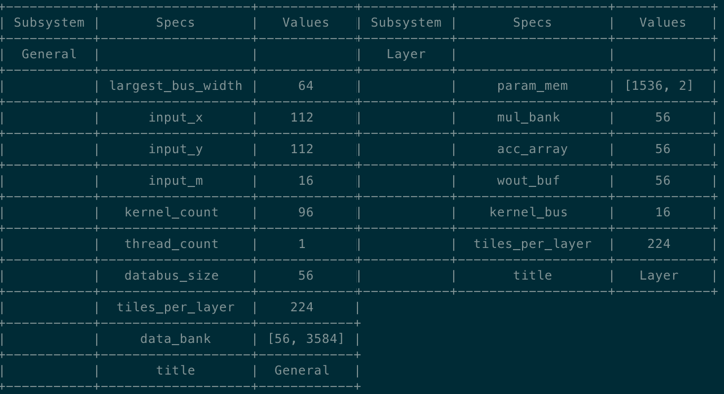
\includegraphics[width=\textwidth]{figures/model_analysis_output}
\caption{Sample output of model analysis}\label{fig:model_analysis_output}
\end{figure}

\subsection{RTL Library Implementation}

The parameters obtained during model analysis are used to generate hardware processing pipelines of appropriate sizes to execute the \gls{neural_net}. This is achieved through a combination of using parameterized Verilog modules which generate processing banks of specified widths at compile time, and code generation which inserts portions of Verilog which cannot be parameterized (refer to \ref{sec:rtl_gen}).

While the Verilog code of a single processing element such as an adder or a multiplier is trivial, the complexity of generating a large-scale \gls{neural_net} processing system is in connecting, controlling, and scheduling these processing elements. Some portions of the processing pipeline are organized into `banks' of parallel processing elements, such as adders and accumulators. These structures can be generated at \gls{rtl} compile time using Verilog parameters which are filled in using the output values of model analysis.

Listing \ref{lst:verilog_gen} shows the Verilog code for generating a bank of 8-bit multipliers. The only parameter which needs to be replaced is `NUM\_MULTIPLIERS' on line 2, corresponding to `mul\_bank' from the output of model analysis in Figure \ref{fig:model_analysis_output}. A generate block in Verilog generates an array of multipliers, which are connected to portions of the input and output vectors of the bank. This array of multipliers multiplies each 8-bit segment of its input vector with a \gls{weight} (input b), corresponding to the multiply operation of a 1x1 \gls{kernel}. The same structure extends to larger \gls{kernel} dimensions.

\begin{figure}
\centering
\begin{lstlisting}[caption={Verilog compile-time generation}, label=lst:verilog_gen, language=Verilog]
module multiplier_bank  #(
    parameter NUM_MULTIPLIERS = 56,
    parameter WIDTH_BITS_IN = NUM_MULTIPLIERS*8,
    parameter WIDTH_BITS_OUT = NUM_MULTIPLIERS*16
)
(
    input [WIDTH_BITS_IN-1:0]           a,
    input [7:0]                         b,
    output signed [WIDTH_BITS_OUT-1:0]  out
);

genvar i;
generate
    for (i=0; i<NUM_MULTIPLIERS; i=i+1) begin: mult
        mult mult (
            .a( a[ (i+1)*8 - 1 : i*8 ] ),
            .b( b ),
            .out( out[ (i+1)*16 - 1 : i*16 ] )
        );
    end
endgenerate
endmodule
\end{lstlisting}
\end{figure}

This type of implementation results in Verilog native hardware generation support, with the only code generation needed being the changing of the parameter. Since Verilog further supports passing parameters through the hierarchy, only the top-level Verilog file would need to contain the editing fields for the parameters. The structure allows individual hardware modules such as a multiplier to be unit-tested and ensures that code generation would not result in non-compilable code. The generation functionality of the bank can also be guaranteed.

Another critical aspect of the hardware structure is the scheduling of the processing pipelines and memory addresses. To maintain identical functionality with a CPU implementation of the same network, memory addresses and control signals need to be correctly generated from the base values in the microcode so that the correct inputs are fed to the multipliers and accumulation is correctly performed.

Listing \ref{lst:sequencer_fsm_1} contains sections of abbreviated code from a sequencer state machine for 1x1 convolutions. The state machine contains the counting logic to iterate through the four loops outlined in \ref{sec:scheduler}. In this sequencer state machine, the `CH\_LOOP' state starting at line 206 contains the counting logic and control signal generation to accumulate multiplication results over all input channels. The address offset registers used in lines 18 and 19 stores the offset values to add to the base address in the microcode to obtain the correct set of data. Loop counters are compared to microcode base values (such as in line 13) to correctly loop over the input \glspl{tensor} and \glspl{kernel}.

\begin{figure}
\centering
\begin{lstlisting}[caption={Sequencer state machine part 1}, label=lst:sequencer_fsm_1, language=Verilog, escapechar= numbers=left, firstnumber=201]
IDLE: begin
   // wait to start loop
end

CH_LOOP: begin                // loop over all input channels
   pipeline_rstn_next = 1'b1; // unreset the pipeline
   mult_enable_next   = 1'b1; // enable multipliers
   acc_en_next        = 1'b1; // enable accumulation
   ...

   if (reg_channel_count == NUM_INPUT_CHANNELS-1) begin
       // finished accumulation over all input channels, write out current tile
       next                  = WR_OUT;
   end else begin
       // haven't finished accumulation, read next input channel to accumulate
       // add offset to read address
       in_ch_offset_next     = reg_in_ch_offset + NUM_TILES;
       // add offset to kernel address
       kernel_ch_offset_next = reg_kern_ch_offset + 1;
       // increment channel counter
       channel_count_next    = reg_channel_count + 1;
       // continue looping
       next                  = CH_LOOP;
   end
\end{lstlisting}
\end{figure}

Listing \ref{lst:sequencer_fsm_2} contains the last state of the sequencer state machine. The `WR\_OUT' state contains the logic to issue write out signals to the pipeline the memory and to re-evaluate the next memory base addresses to read from. Depending on the size of the layer, the number of iterations required for the pipeline to accumulate all the results required to write out differs. Again, the microcode contains the parameters specifying the number of loops.

\begin{figure}
\centering
\begin{lstlisting}[caption={Sequencer state machine part 2}, label=lst:sequencer_fsm_2, language=Verilog]
WR_OUT: begin
    // issuing writeout
    pipeline_rstn_next          = 1'b0; // reset the pipeline
    acc_en_next                 = 1'b0; // disable accumulation
    ...
    data_mem_wr_en_next         = 1'b1; // enable writeback memory

    // reset the channel offsets and counters
    channel_count_next          = 0;
    kernel_ch_offset_next       = 0;
    in_ch_offset_next           = 0;

    if (reg_kernel_count == NUM_KERNELS) begin
        next                    = IDLE;
    end else if (reg_tile_count == NUM_TILES-1) begin
        // finished full image, do next kernel
        next                    = CH_LOOP;
        // increment kernel counter
        kernel_count_next  = reg_kernel_count + 1;
        // reset tile count
        tile_count_next    = 0;
        // kernel addr offs
        kernel_offset_next = reg_kernel_offset + NUM_INPUT_CHANNELS;
        // data addr offset
        out_ch_offset_next = reg_out_ch_offset + NUM_TILES;
        tile_offset_next   = 0;
    end else begin
        // not done image,  at next tile and loop again
        next               = CH_LOOP;
        tile_offset_next   = reg_tile_offset + 1;
        tile_count_next    = reg_tile_count + 1;
    end
end
\end{lstlisting}
\end{figure}

When the processing pipeline has finished accumulating, the state machine issues a write out address and enable to the memory, and the output of the pipeline is written to memory at the generated address. In this state, the loop variables are re-evaluated to arrive at the correct set of parameters with which to start the next loop. The inner loop counters and address offsets are reset, and the state returns to `CH\_LOOP' until every \gls{kernel} has been processed.

This sequence of operations reflects the loops outlined in \ref{sec:scheduler}, with the innermost loop (for weights in \gls{kernel}) fully unrolled, and the second loop (for input pixel/value in image/volume) partially unrolled. This matches the hardware system design in \ref{sec:top_level_framework} and \ref{sec:macro_gen}, optimizing for limited on-chip memory and maximizing data reuse.

Figure \ref{fig:rtl_simulation_waveform} shows example waveforms from \gls{rtl} simulation of the sequencer and macro block implementing a 1x1 convolution. All signals and busses showing the flow and computation of data is shown from top-to-bottom, starting by loading one frame from main memory and ending by writing back to a different location in memory.

\begin{figure}
\centering
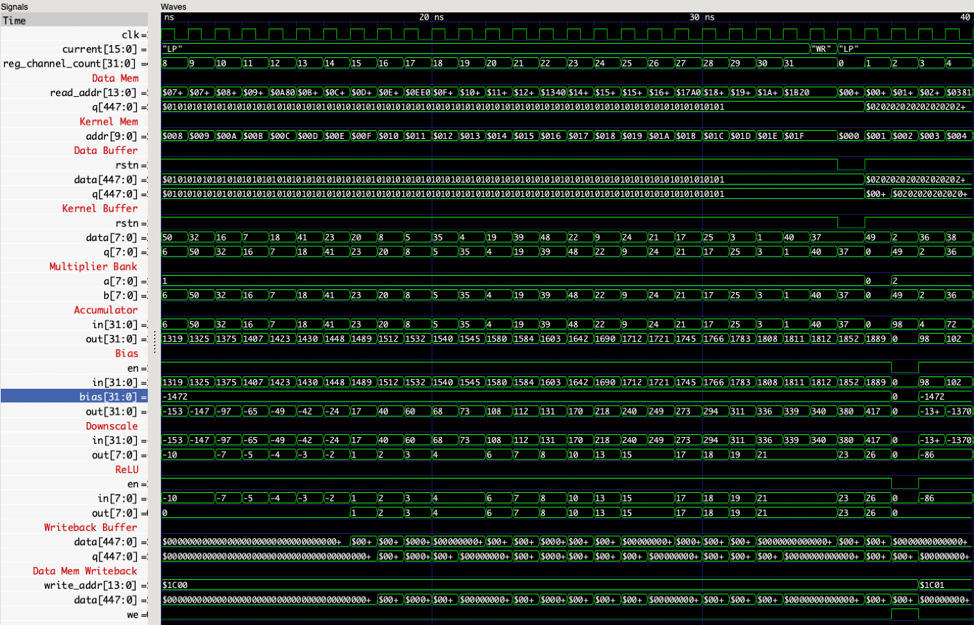
\includegraphics[width=\textwidth]{figures/rtl_simulation_waveform}
\caption{\Gls{rtl} simulation waveform for toy 1x1 convolution hardware}\label{fig:rtl_simulation_waveform}
\end{figure}

After \gls{rtl} simulation, a dump of main memory can be obtained and compared with the output of the functional model for verification. This allows cross-comparison at three levels of abstraction: the ground truth output of TensorFlow, the operation-accurate functional Python implementation, and the final \gls{rtl} implementation.

\section{Discussion and Conclusions}

\subsection{Evaluation of Final Design}

The final design of this project effectively meets all the specifications and goals initially set by the team. The user interface is designed such that the users can easily specify constraints (memory usage, \gls{le} count, etc.) and the model using a configuration file.

The user specified model is ingested through the TensorFlow API as a directed acyclic graph representation for use in the rest of the system. The graph is then analyzed accurately using the GraphDef interface to extract model properties, such as operations, dimensions of input and output channels, etc. The model can be compressed effectively using quantization and pruning of zero weights through graph transforms in TensorFlow Lite. After compression, the optimization steps and the optimized model are returned to the user for transparency in the process. The fixed-point representation provided by model compression reduces the \gls{le} count required significantly because of the reduced bit width compared to floating-point weights.

\gls{fpga} space constraints by addressed by designing hardware architecture that is flexible and scalable to nets of various sizes. A shared-multiplier architecture was chosen for its efficient hardware usage and ability to fit large models.

Finally, and most importantly, this design allows for functional correctness of the hardware components. The hardware macros used to build the hardware representation have been shown to be accurate from academia. Additionally, due to the deterministic nature of the mapping from TensorFlow graph nodes to hardware macros, the synthesizable \gls{rtl} output of the system is expected to be functionally accurate.

\subsection{Use of Advanced Knowledge}

This project utilizes advanced knowledge from both electrical and computer engineering. The hardware design of a \gls{cnn} accelerator is extremely challenging and generally spans advanced graduate-level knowledge or relevant industry background. Past work in this field exploring architectural design decisions was produced primarily by teams in \gls{vlsi} research groups from various institutions world wide.

The digital implementation of the accelerator requires a broad understanding of pipelining, parallelization, memory interfaces, caches, buses, and \gls{fpga} logic elements. It also requires deep technical experience in \gls{rtl} implementation, simulation, timing closure, and verification. These concepts are explored at a basic level in courses such as Embedded Computer Systems (ECE 423) and Computer Architecture (ECE 429) and are covered to a more rigorous depth in graduate courses such as Computational Organization (ECE 621), RTL Digital Systems (ECE 627), and Reconfigurable Computing (ECE 722).

The project also requires an advanced understanding of state-of-the-art \glspl{neural_net} and their operation to be able to break down network elements into pre-defined hardware blocks. An understanding of autonomous vehicles and their functions is also required to create a design that can integrate with these systems. The necessary background in machine vision, convolutional \glspl{neural_net}, semantic segmentation networks, and autonomous vehicles, is introduced in Technical Electives such as Fundamentals of Computational Intelligence (ECE 457B) and Autonomous Vehicles (ECE 493 Topic 21).

Additionally, our team is relying heavily on relevant experience from working in industry and vehicle design teams as a substitute for the formal graduate-level training normally required to be able to undertake a project of this scope and difficulty.

\subsection{Creativity, Novelty, Elegance}

This work builds heavily on existing research in \gls{fpga} acceleration schemes for \glspl{cnn}. A significant amount of time was spent surveying various published works describing different architectures \cite{Cheng2018Model-Compressi}. While a wealth of research exists relating to traditional \glspl{cnn} for image recognition, little to no research exists relating to semantic segmentation models.

Image segmentation is a critical concept in the development of autonomous driving and for these reasons, traditional image recognition nets, for which research in this area current exists, cannot be directly applied to machine vision challenges for autonomous vehicles. The primary focus of our work is to create a dynamic architecture capable of implementing segmentation nets and optimizing its performance in a real vehicle, as part of WATO's design goals. These state-of-the-art networks will be in use in the next generation of autonomous vehicles due to their precision, allowing for better understanding of a vehicle's environment \cite{Chen2019Importance-Awar}. This involves several new challenges, as segmentation networks are structured differently than traditional image nets and involve new types of computational layers for decoding a classification back into a pixel-by-pixel mapping. Implementing hardware for \glspl{fpga} enables both immediate practical deployment in vehicles and creates a technical foundation for porting such a design to application specific integrated circuits.

This solution also leverages TensorFlow, an existing standard in \gls{neural_net} description that is very widely used and allows for the seamless conversion to optimized and functional hardware that will perform significantly better than traditional execution units such as a CPU. All of this is achieved through a simple and easy to use user interface that can be integrated with fast-paced \gls{neural_net} development workflows.

\subsection{Quality of Risk Assessment}

The risk assessment completed in ECE 498A was instrumental in reducing the risks to the project. The team was able to mitigate and work around issues and problems we faced throughout the project. The integration with WATonomous has had its challenges, as predicted previously. There were difficulties with communication as there were changes of communication platforms and management during the project. To mitigate this issue, the team met with team leads often to sync up in person and online. It allowed both sides to work together well.

The risk we identified with the WATO team's model complexity was mitigated by defining that the project will support a specific subset of operations\textemdash{}the ones present in MobileNet. This allowed both parties to continue working on the project separately and integration was relatively seamless. There were only a few issues with file formats, rather than fundamental design issues.

Group member availability issues were mitigated by frequent sync ups and meetings that allowed all members to have blocked times in their calendar to work together on issues at hand.

To mitigate the lack of access to hardware and software tools, the team obtained separate sponsorship for an Intel Arria 10 \gls{fpga} dev board and Quartus development tools. Our development and build computer was placed on the Google Cloud Platform to allow us to have high power and optimized build machines on demand, at a reasonable cost. This allows us to work independently and have 24/7 access to the hardware and software.

\subsection{Student Workload}

This project was contributed to equally by each member of the team. The workload is therefore equivalent between all members as seen in Table \ref{tab:student_workload}.

\begin{table}[hbp]
\centering
\caption{Student workload distribution}\label{tab:student_workload}
\begin{tabular}{lc}
\toprule
Group Member         & Percentage of Overall Workload \\
\midrule
Pragash Sivasundaram & 20\% \\
Timothy Chee Tim Mui & 20\% \\
Minghao Ji           & 20\% \\
Tong Su              & 20\% \\
Yifei Li             & 20\% \\
\bottomrule
\end{tabular}
\end{table}

%%%%%%%%%%%%%%%%%%%%%%%%%%%%%%%%%%%%%%%%%%%%%%%%%%%%%%%%%%%%%%%%%%%%%
%% BACK MATTER
%%%%%%%%%%%%%%%%%%%%%%%%%%%%%%%%%%%%%%%%%%%%%%%%%%%%%%%%%%%%%%%%%%%%%
%% \backmatter will make the \section commands ignore their numbering,
\backmatter

\begin{refsection}
\printglossaries
\end{refsection}
\newpage
\printbibliography
\addcontentsline{toc}{section}{References}

%%%%%%%%%%%%%%%%%%%%%%%%%%%%%%%%%%%%%%%%%%%%%%%%%%%%%%%%%%%%%%%%%%%%%
%% APPENDICES
%%%%%%%%%%%%%%%%%%%%%%%%%%%%%%%%%%%%%%%%%%%%%%%%%%%%%%%%%%%%%%%%%%%%%
%% \appendix will reset \section numbers and turn them into letters.
%%
%% Don't forget to refer to all your appendices in the main report.
\appendix



\end{document}
